
\section{Higher-Order Test Cases}

The higher-order test cases are designed to test various aspects of higher-order dycores.
By default they all use the Glissade dycore.  Other higher-order dycores can be applied
to these tests as they become available.

% =====================================
\subsection{Dome}
% =====================================
The ``Dome'' test case is an ellipsoidal dome of ice similar to the Halfar dome test case.
By default the Dome has the same radius and the same center thickness as the Halfar case.
However, it uses a simple square root function for defining thickness as a function 
of distance from the dome center which results in a somewhat steeper profile.  
The Dome has been the primary test used for day-to-day testing of higher-order
test cases because it is simple and relatively fast to run.  It is a good test
to confirm that basic higher-order model physics is working correctly, but does
not strenuously test the model or analytically verify the model.

\subsubsection{Provided Files}

\begin{itemize}
	\item README \\
		Information about the test case, including technical details about running it.
	\item dome.py \\
		The script to setup and run the test test.
  \item dome.config \\
  The default configuration settings for running CISM with the test case.
	\item dome.forcing.py \\
		A optional script for setting up an example of a CISM time-dependent forcing file.
  \item dome.forcing.config \\
  An example configuration script that can be used to run CISM with the forcing file
  generated by \texttt{dome.forcing.py}
\end{itemize}

\subsubsection{Running the test}
One script sets up the initial condition and runs the model:

\texttt{./dome.py}

There is not a script for analyzing the results.

\textit{Optional:  Time-dependent forcing example}

The Dome test case can be used to setup an example of how to use CISM's time-dependent
forcing capability.  (See Section \ref{ug.sec.config} for more details about time-dependent
forcing.)  To create a forcing file with some time-varying (though arbitrary) forcing, run:

\texttt{./dome.forcing.py}

Then you can run the model using the \texttt{dome.forcing.config} configuration file:

\texttt{./dome.py -c dome.forcing.config}

or

\texttt{./cism\_driver dome.forcing.config}


\subsubsection{Results}
There is not an analytic solution for this test, nor is there a script to analyze
the results.  You can manually inspect the results using a tool such as \texttt{ncview}.
An example is shown in Figure \ref{fig:domeresults}.
\textbf{SP: we need to clarify that this is a time dependent problem and which time step is shown in the figure.}
\begin{figure}[H!]
	\centering
	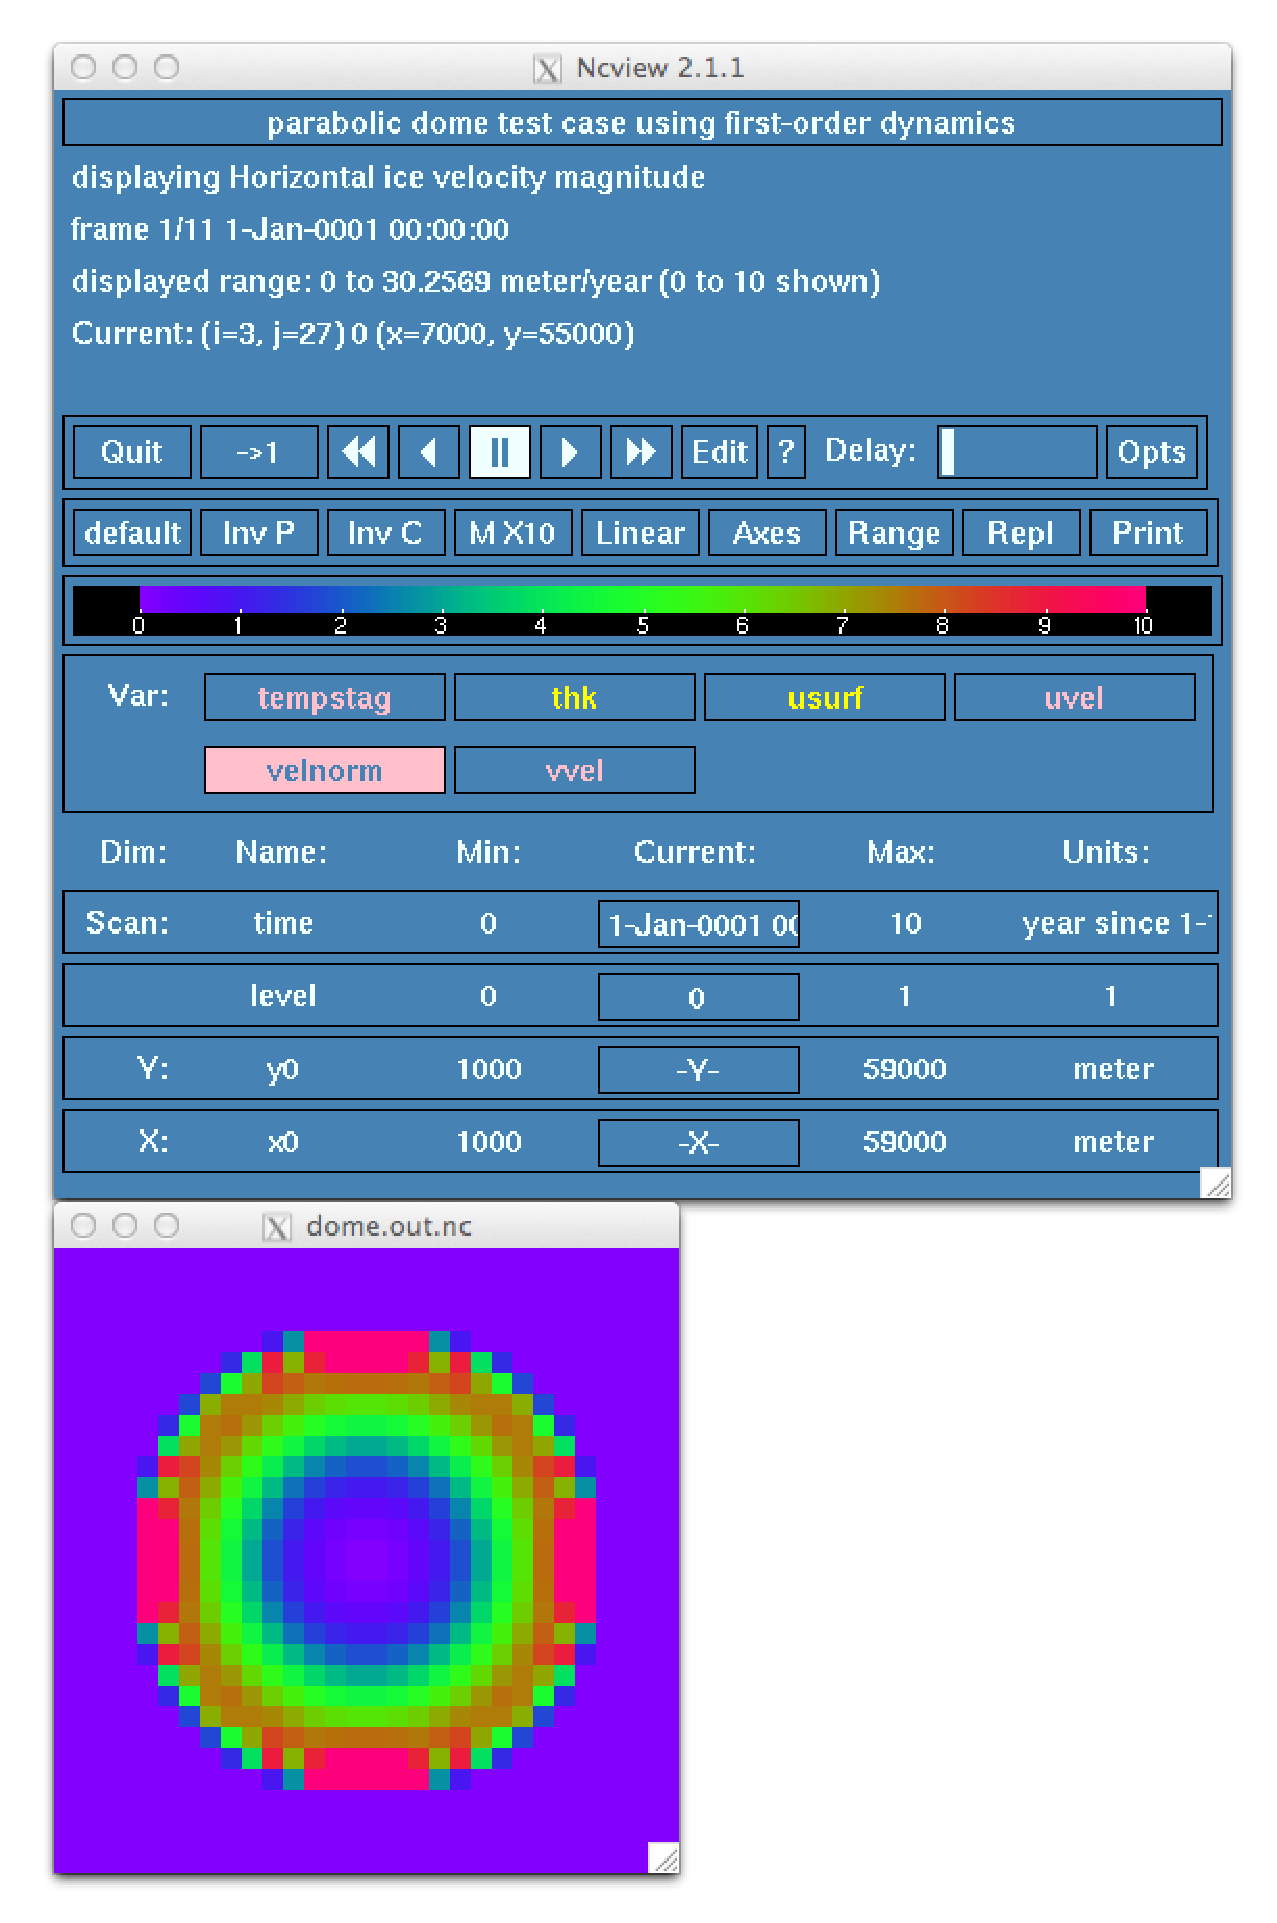
\includegraphics[width=8.0cm]{\dir/dome-output.eps}
	\caption{Dome velnorm field at time 0 using default \texttt{dome.config} settings. This figure is a screenshot of ncview.}
	\label{fig:domeresults}
\end{figure}
\FloatBarrier

% =====================================
\subsection{ISMIP-HOM}
% =====================================
Ice Sheet Model Intercomparison Project for Higher-Order Models (ISMIP-HOM)
prescribes a set of experiments meant to test the implementation of
higher-order physics.  For more information, see
\url{http://homepages.ulb.ac.be/~fpattyn/ismip/} and the ISMIP-HOM description paper
by \citet{Pattyn2008}.

The python scripts provided (runISMIPHOM.py and plotISMIPHOM, refered to
in the following as the ISMIP-HOM scripts) were created to run the experiments
using Glimmer/CISM and compare the results with results from other models.

Note: The \texttt{README} file describes many details about running and analyzing the
test case that are not described here.

\subsubsection{Provided Files}

\begin{itemize}
	\item README \\
		Information about the test case, including technical details about running it.
	\item ishom.config \\
		A default configuration file used as a template for generating the .config file for each test.
    If you wish to run the tests with different solver settings, for example, you should edit this file.
	\item runISMIPHOM.py \\
		The script used for running any/all of the ISMIP-HOM experiments.  
    Invoke with --help to see the many command line options for controlling execution.
  \item plotISMIPHOM.py \\
		The script used for analyzing/plotting any/all of the ISMIP-HOM experiments.  
    Invoke with --help to see the many command line options for controlling execution.
\end{itemize}

\subsubsection{Running the test}
One script sets up the initial condition and runs the model:

\texttt{./runISMIPHOM.py}

and another is used to analyze the results:

\texttt{./plotISMIPHOM.py}

\subsubsection{Results}
The \texttt{plotISMIPHOM.py} script will plot results relative to other models.
None of the ISMIP-HOM tests have a useful analytic solution, so these tests are
used as community benchmarks rather than actual model verification tests.
Therefore, the \citet{Pattyn2008} paper is useful for intepreting model results.
An example output plot is shown in Figure \ref{fig:ismiphom-results}.


\begin{figure}[H!]
	\centering
	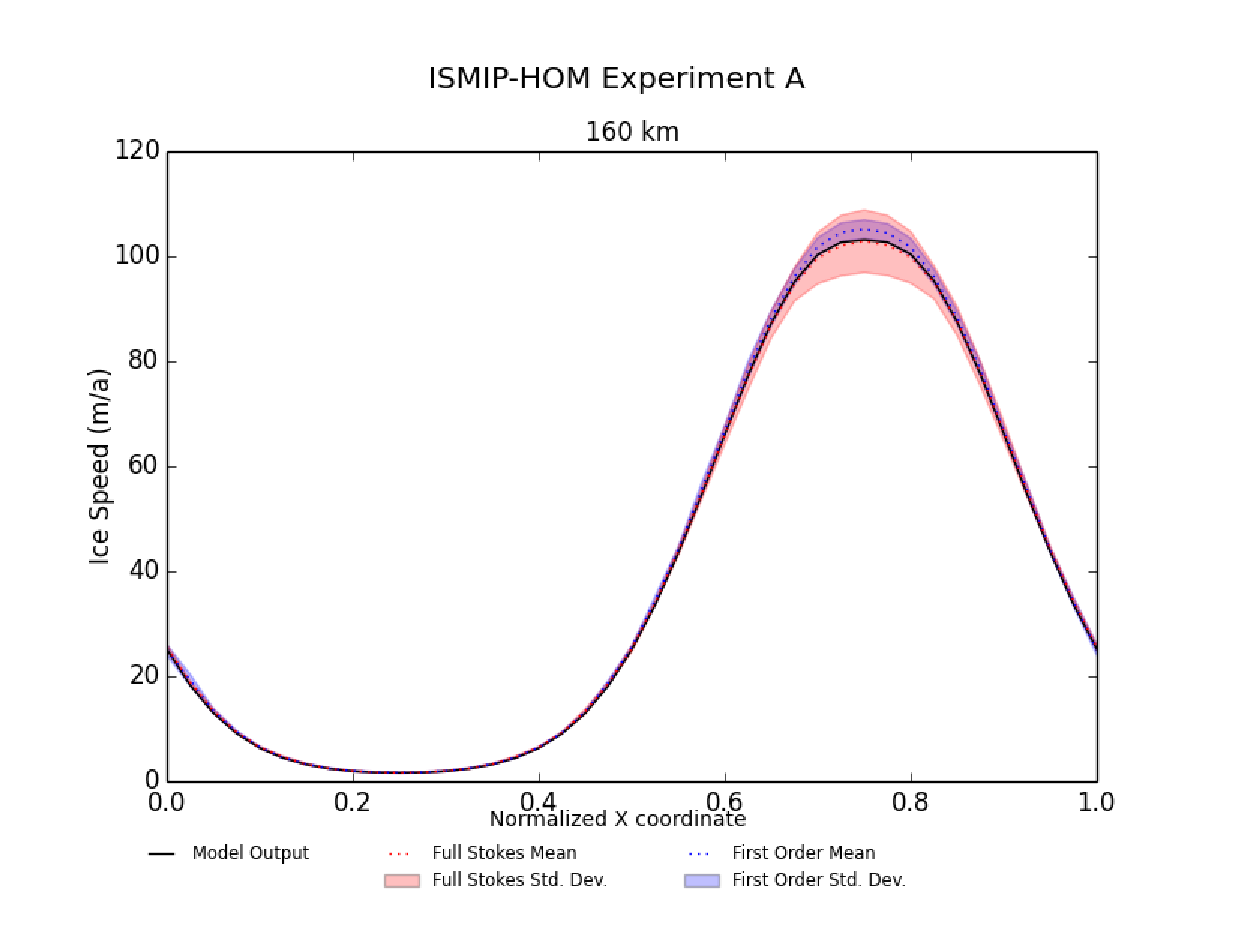
\includegraphics[width=12.0cm]{\dir/ISMIP-HOM-A-cis1.eps}
	\caption{An example of the ISMIP-HOM test case output for test A at size L=160 km. 
CISM output is shown with black line and the range of output from other models is shown by colored bars. 
This figure was generated with \texttt{./plotISMIPHOM.py -e a -s 160} after running the test with \texttt{runISMIPHOM.py -e a -s 160}}
	\label{fig:ismiphom-results}
\end{figure}
\FloatBarrier

% =====================================
\subsection{Confined Shelf}
% =====================================
This test setup is from tests 3 and 4 from the more "simple"
(i.e. not Ross) EISMINT-shelf test cases.  It tests an idealized ice shelf in a 
confined embayment.  Grounded ice is not explicitly modeled but included in the 
model setup as Dirichlet boundary conditions for velocity along the ice shelf edges.
Detailed information on this test can be found at:
\url{http://homepages.vub.ac.be/~phuybrec/eismint/iceshelf.html}
in the shelf-descr.pdf document.

Note that the Confined Shelf and Circular Shelf experiments are both in the 
\texttt{tests/higher-order/shelf} directory and share some files.

\subsubsection{Provided Files}

\begin{itemize}
	\item README \\
		Information about the test case, including technical details about running it.
	\item confined-shelf.py \\
		The script to setup and run the test test.
	\item confined-shelf.config \\
  The default configuration settings for running CISM with the test case.
\end{itemize}

\subsubsection{Running the test}
One script sets up the initial condition and runs the model:

\texttt{./confined-shelf.py}

\subsubsection{Results}
There is not a script for analyzing the results.  See the URL above for information 
about assessing the model output.
You can manually inspect the results using a tool such as \texttt{ncview}.
An example is shown in Figure \ref{fig:confinedshelf-results}.

\begin{figure}[H!]
	\centering
	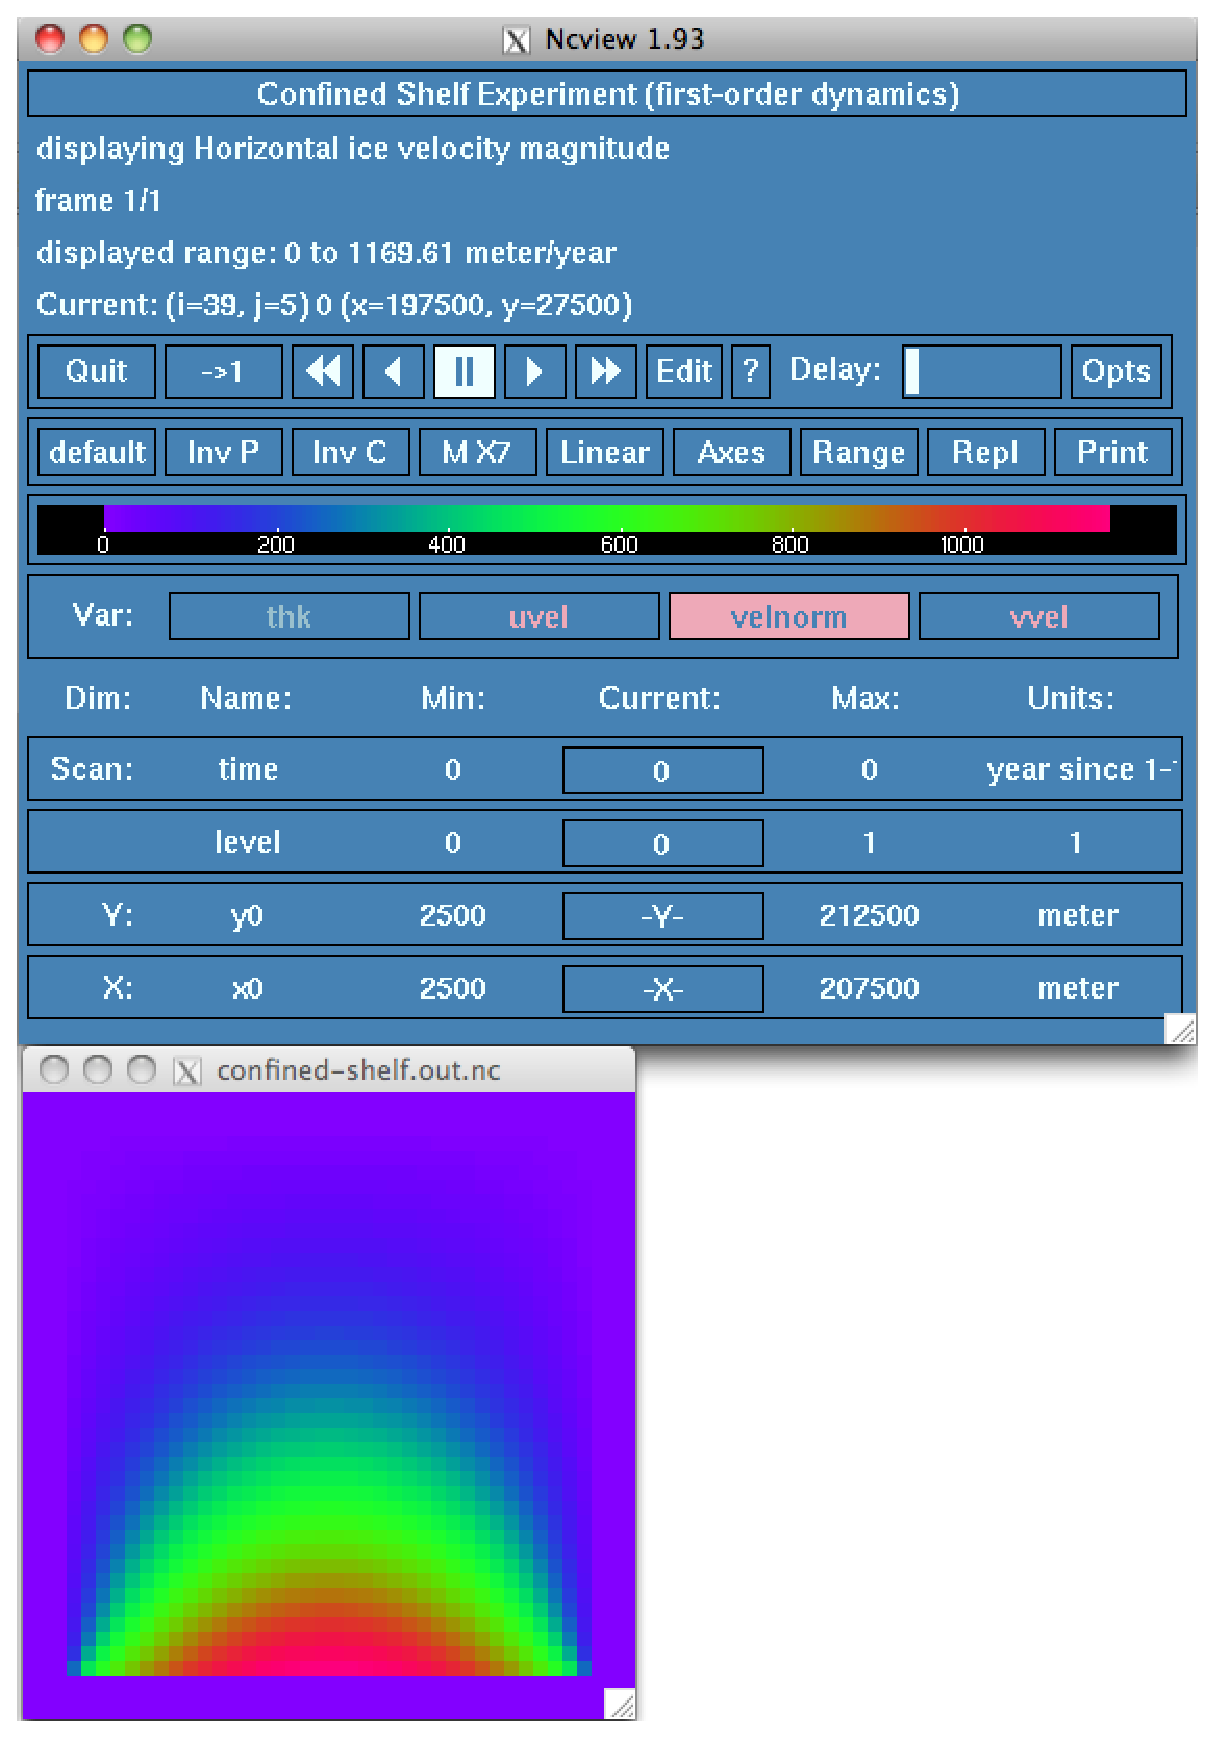
\includegraphics[width=8.0cm]{\dir/confinedshelf-output.eps}
	\caption{Confined shelf velnorm field using default \texttt{confined-shelf.config} settings. This figure is a screenshot of ncview.}
	\label{fig:confinedshelf-results}
\end{figure}
\FloatBarrier

% =====================================
\subsection{Circular Shelf}
% =====================================
This test models a circular ice shelf that is grounded at single point in the center
of the shelf.  It tests 

Note that the Confined Shelf and Circular Shelf experiments are both in the 
\texttt{tests/higher-order/shelf} directory and share some files.

\subsubsection{Provided Files}

\begin{itemize}
	\item README \\
		Information about the test case, including technical details about running it.
	\item circular-shelf.py \\
		The script to setup and run the test test.
	\item circular-shelf.config \\
  The default configuration settings for running CISM with the test case.
\end{itemize}

\subsubsection{Running the test}
One script sets up the initial condition and runs the model:

\texttt{./circular-shelf.py}

\subsubsection{Results}
There is not a script for analyzing the results.
You can manually inspect the results using a tool such as \texttt{ncview}.
An example is shown in Figure \ref{fig:circularshelf-results}.

\begin{figure}[H!]
	\centering
	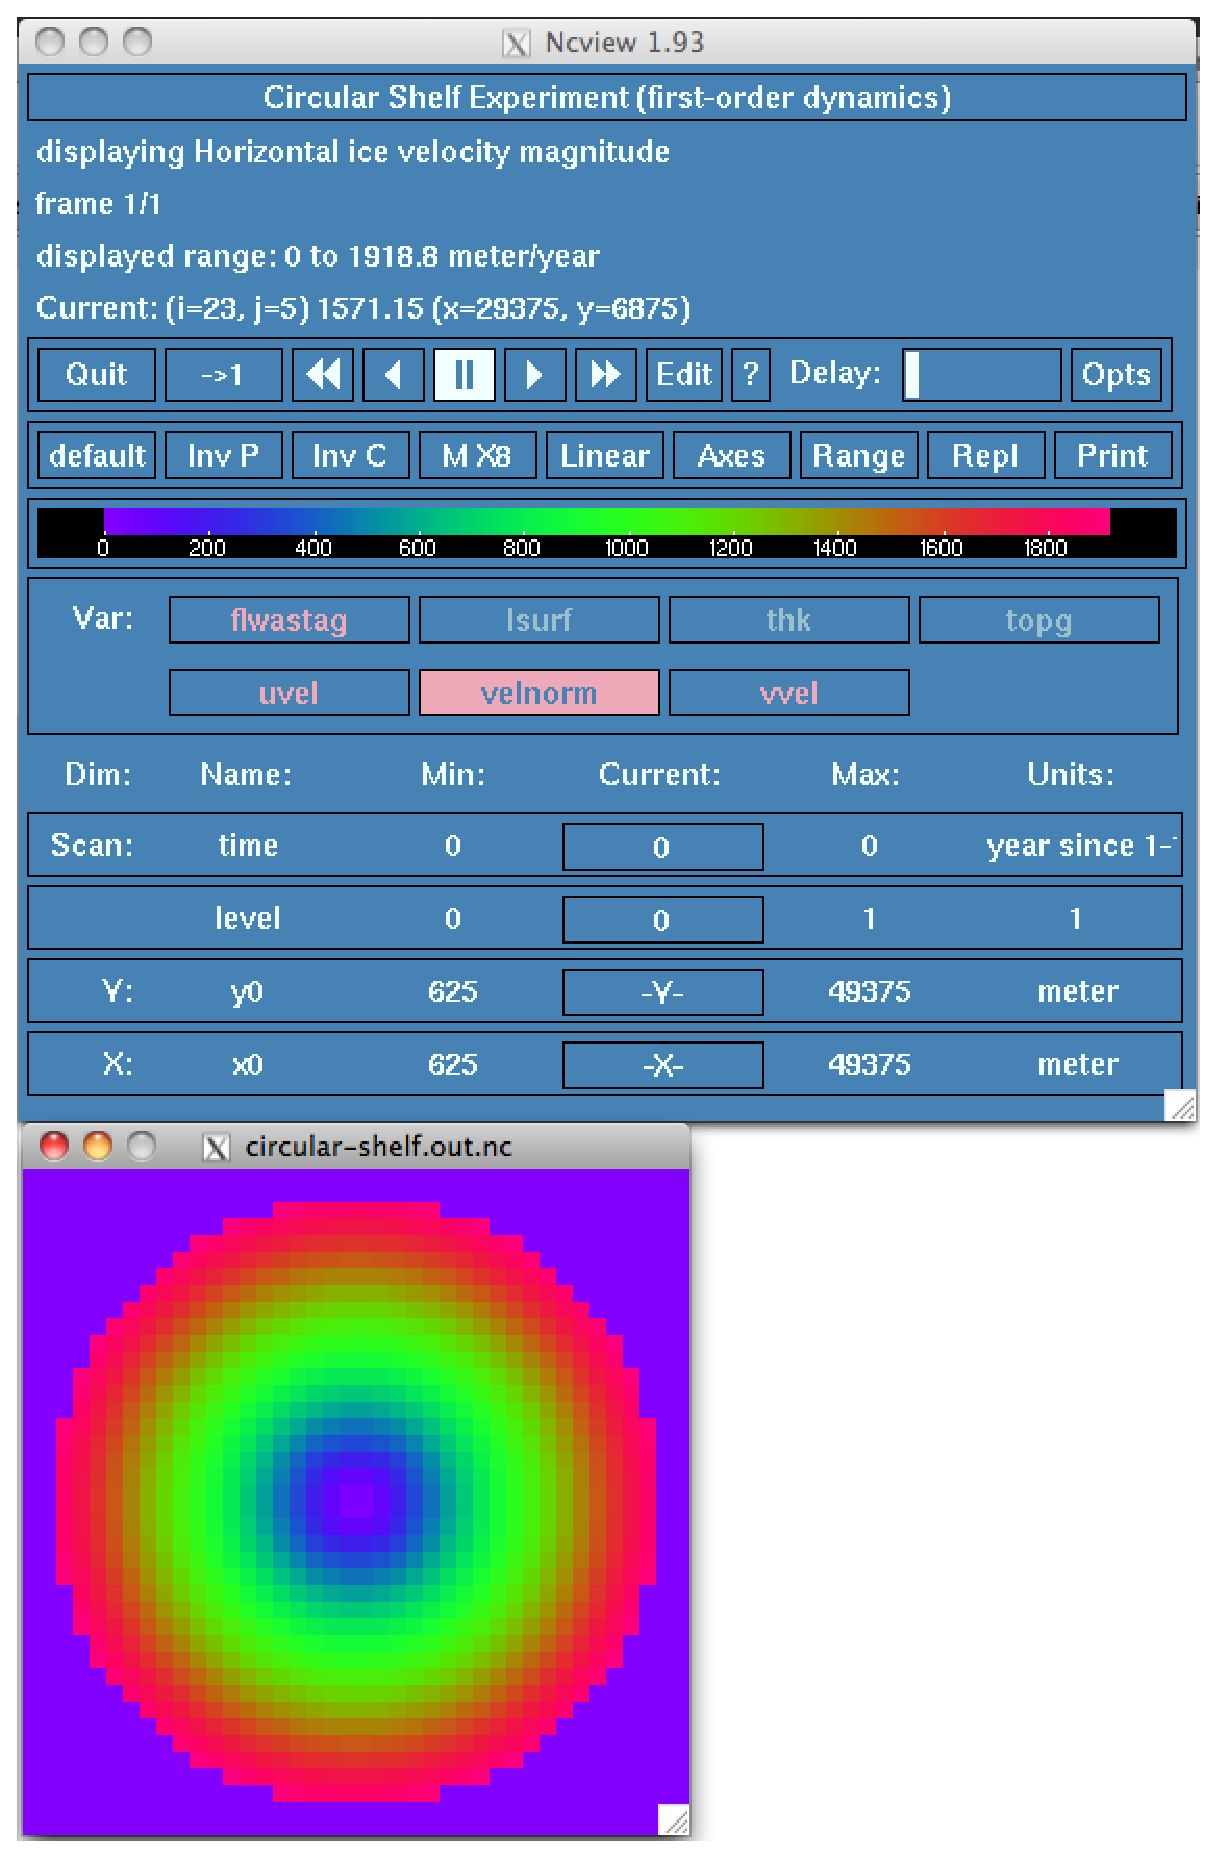
\includegraphics[width=8.0cm]{\dir/circularshelf-output.eps}
	\caption{Circular shelf velnorm field using default \texttt{circular-shelf.config} settings. This figure is a screenshot of ncview.}
	\label{fig:circularshelf-results}
\end{figure}
\FloatBarrier

% =====================================
\subsection{Ross Ice Shelf}
% =====================================
This experiment was designed to model the Ross Ice Shelf of Antarctica.
For information about the experiment and its results see:
\url{http://homepages.vub.ac.be/~phuybrec/eismint/iceshelf.html}

This experiment will typically take about 10 minutes on a single processor.

\subsubsection{Provided Files}

\begin{itemize}
	\item README \\
		Information about the test case, including technical details about running it.
	\item runRoss.py \\
		The script to setup and run the test test.
	\item ross.config \\
  The default configuration settings for running CISM with the test case.
	\item plotRoss.py \\
		The script to plot the test results.
\end{itemize}

\subsubsection{Running the test}
One script sets up the initial condition and runs the model:

\texttt{./runRoss.py}

and another can be used to visualize the results:

\texttt{./plotRoss.py}

\subsubsection{Results}
The \texttt{plotRoss.py} script will generate a figure of the velocity field
calculated for the Ross Ice Shelf.  The result should look very similar to to Figure \ref{fig:rossresults}.

\begin{figure}[H!]
	\centering
	%\includegraphics[width=8.0cm]{\dir/ross_results.eps}
	\caption{Ross Ice Shelf velocity field calculated by CISM. This figure is generated by \texttt{plotRoss.py}.}
	\label{fig:rossresults}
\end{figure}
\FloatBarrier


% =====================================
\subsection{Other Tests}
% =====================================
Additional higher-order tests are in development (slab, stream).  Instructions
for how to run them are in each directory, but these tests have not yet been 
scientifically validated, so use at your own risk.


